\documentclass[../main.tex]{subfiles}

\begin{document}

\section{Introduction}

\subsection{Bacterial Chemotaxis as a Model System}
The benefits of using model organisms in biology are comprehensive. In the field of systems biology, we move a step deeper and study model systems. Amongst them, bacterial chemotaxis in \ecolilong is one of the most extensively studied. The stoichiometry is well established~\citep{li04}, the structure of all major constituent proteins have been determined~\citep{zhou02, milligan87, stock89}, and the feedback loops involved described~\citep{kentner09} and robustness tested~\citep{yi00}. The \ecoli system has also been used as the basis for study of chemotaxis in other bacteria{hamadeh11}.

In more recent times with the advent of more and more powerful computers, chemotaxis in \ecoli has presented itself as an ideal target for the development of advanced simulations~\citep{bray93, lipkow05, miller10}, allowing researchers to postulate new and more detailed mechanisms of control. Together with advances in high resolution microscopy~\citep{greenfield09} this has opened the door to new insights into the behaviour of the \ecoli chemotaxis network.

The outcome of this research is the following model of chemotaxis (Figure~\ref{fig:chemo:bubble}):

\paragraph{Transmembrane Methyl-accepting chemotaxis proteins} (MCPs) sit in a cluster at one or both poles of the cell. The presence of repellents or attratants is tranduced through a piston like motion~\citep{hall11}. Each MCP has four methylation sites. The level of transduction of the signal through the MCP is modulated by the number of methylated sites. MCP activity is increased by repellent and decreased by attractant, and more methyl sites give better transduction.

\paragraph{CheA and CheW proteins} sit at the base of the MCPs. CheA is a histidine kinase, and in its active form may autophosphorylate in response to a transduced signal from an MCP \citep{sourjik10}.

\paragraph{CheB and CheR proteins} are a methylesterase and a methyltransferase, respectively. CheR binds loosely to the MCPs and constitutively adds methyl groups to them. CheB, which diffuses freely, must first receive a phosphate group from phosphorylated CheA (CheAp) before it may remove a methyl group from the MCPs. Thus a negative feedback loop is formed, whereby an increase in MCP activity will cause methyl groups to be removed from the MCPs, thus decreasing their efficacy in transducing signals.

\paragraph{CheY protein} diffuses freely throughout the cell, and is the messenger protein responsible for carrying information from the polar clusters to the motor clusters. It carries this information by receiving the phosphate group from CheAp.

\paragraph{Motor clusters} are located at various points along the side of the cell, and usually number between 5 and 8 \citep{wadhams04}. A complex bi-stable like system regulates the direction of spin of the motor. Normally the motor turns counter clockwise. However, when a critical level of phosphrylated CheY (CheYp) is reached, the motor will spin clockwise, causing a tumble in the bacteria.

\paragraph{CheZ protein} is found diffusing freely throughout the cell and bound to CheA\textsubscript{short} (a truncated form of CheA) at the polar clusters, and dephosphorylates CheZ.

Thus, from beginning to end, a repellent binding to an MCP will cause an increase in CheYp downstream, increasing the chances of the bacteria tumbling. It will also reduce the transduction efficacy of the MCPs, desensitising them to the current level of repellent and allowing them to detect further increases in repellent levels.


\begin{figure}[h!]
\begin{center}
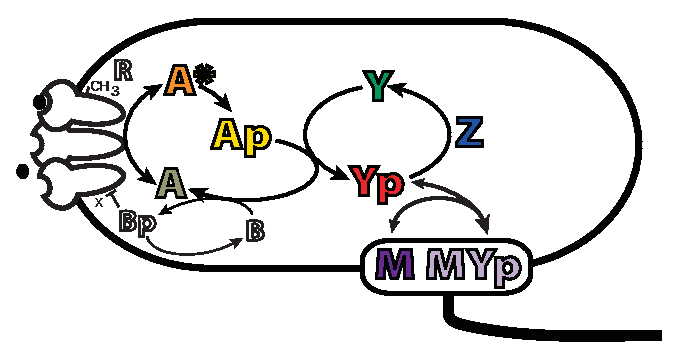
\includegraphics[scale=1]{\docroot introduction/figs/chemotaxis-simple-network}
\caption[Schematic of the chemotaxis system]{Schematic of the chemotaxis system. Note that protein labels are only loosely representative of respective locations in the cell. Figure from \citet{lipkowfigs}.}
\label{fig:chemo:bubble}
\end{center}
\end{figure}

Despite the extensive coverage of research, there are many areas yet to be fully resolved. Amongst these is that simulations of the system above without the methyl feedback do not have the same dynamic range as \ecoli without methyl feedback do; that is, \ecoli can respond to small changes as well at already high concentrations as low concentrations even without the methyl feedback system. Therefore, there must be another feedback loop modulating the chemotaxis response to allow the system to retain sensitivity as concentrations change.

Models of the chemotaxis system in which CheZ clusters at the polar clusters in response to increases in CheYp provide this required dynamic range. The proposed mechanism for this is shown in Figure~\ref{fig:intro:chemo}. An increase in CheZ localised to the polar cluster will decrease global levels of CheYp more effectively than CheZ distributed throughout the cells, giving a negative feedback loop. Simulations of this loop are shown in Figure~\ref{fig:intro:chemo:clusternetwork}, showing that is increases the dynamic range of the system to match that seen in \ecoli~\citep{lipkow06}. To verify this, it is necessary to demonstrate that a greater or lesser proportion of CheZ can be found in the polar clusters while the cell is responding to a chemotactic stimulant, and this task will be the focus of much of this report.

\begin{figure}
\begin{center}
\subfloat[Attractant: low CheYp]{
	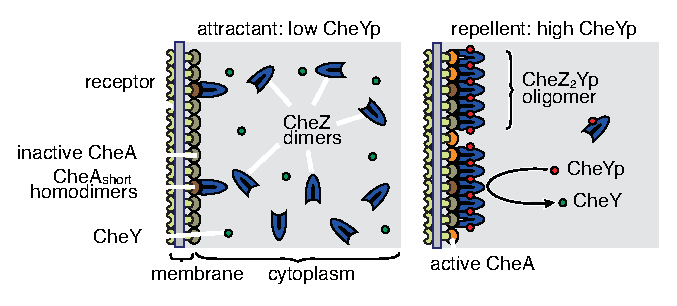
\includegraphics[scale=1, clip=true, trim=0 0 115 12]{\docroot introduction/figs/chezclustering}
	\label{fig:intro:chemo:mech1}
}
\subfloat[Repellent: high CheYp]{
	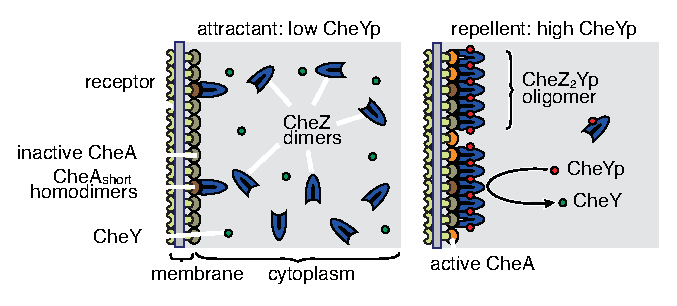
\includegraphics[scale=1, clip=true, trim=190 0 0 12]{\docroot introduction/figs/chezclustering}
	\label{fig:intro:chemo:mech2}
}
\caption[Proposed mechanism of clustering]{Proposed mechanism of clustering, modified from \citet{lipkow06}. In~\subref{fig:intro:chemo:mech1} the presence of an attractant maintains a low level of CheYp, and there is no oligomerisation of CheZ. Some CheZ is bound to CheA\textsubscript{short}. In~\subref{fig:intro:chemo:mech2}, the repellent maintains a high level of CheYp. This allows the CheZ to oligomerise. When one CheZ dimer in an oligomer binds to a CheA\textsubscript{short}, the entire oligomer is kept localised at the cluster.}
\label{fig:intro:chemo}
\end{center}
\end{figure}
\begin{figure}
\begin{center}
\subfloat[Constant CheZ activity]{
	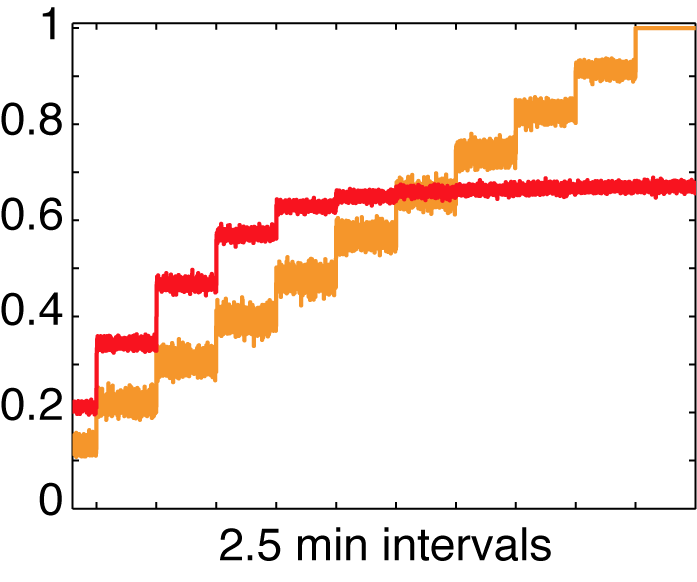
\includegraphics[scale=1]{\docroot introduction/figs/chezactivityold.png}
	\label{fig:intro:chezact:old}
}
\subfloat[Dynamic CheZ activity]{
	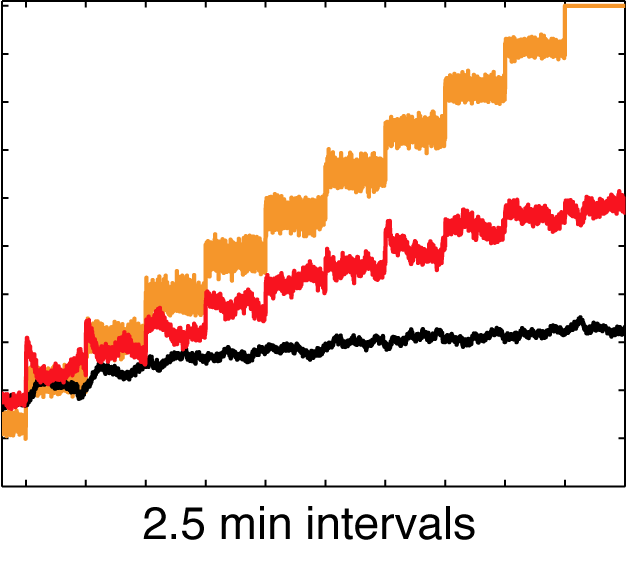
\includegraphics[scale=1]{\docroot introduction/figs/chezactivitynew.png}
	\label{fig:intro:chezact:new}
}
\subfloat{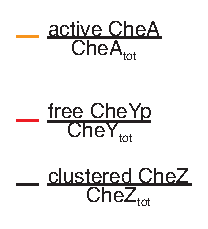
\includegraphics[scale=1]{\docroot introduction/figs/chezactivitykey}}
\caption[Effect of CheZ clustering]{The effect of CheZ clustering, modified from \citet{lipkow06}. In~\subref{fig:intro:chezact:old}, with CheZ not clustering, a series of stepwise increases in CheA activity will eventually saturate the level of CheYp, meaning the cell has no further capacity to deal with increase in repellent. In~\subref{fig:intro:chezact:new}, with CheZ dynamically clustering, the same series of stepwise increases in CheA activity does not cause saturation of CheYp - for each change in the activity of CheA there is a corresponding change in the level of CheYp, allowing the cell to detect changes in repellent even at high basal levels of CheA activity.}
\label{fig:intro:chemo:clusternetwork}
\end{center}
\end{figure}

\begin{figure}
\begin{center}
\subfloat[Canonical chemotaxis network]{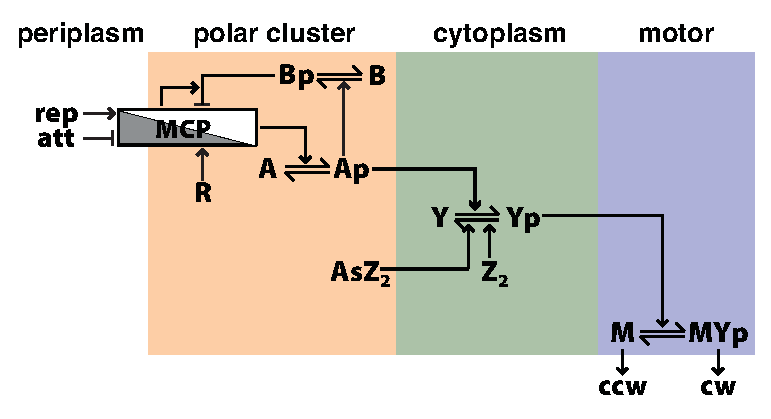
\includegraphics[scale=1]{\docroot introduction/figs/chemotaxis-local-network}}\\
\subfloat[Chemotaxis network with hypothesised CheZ feedback loop]{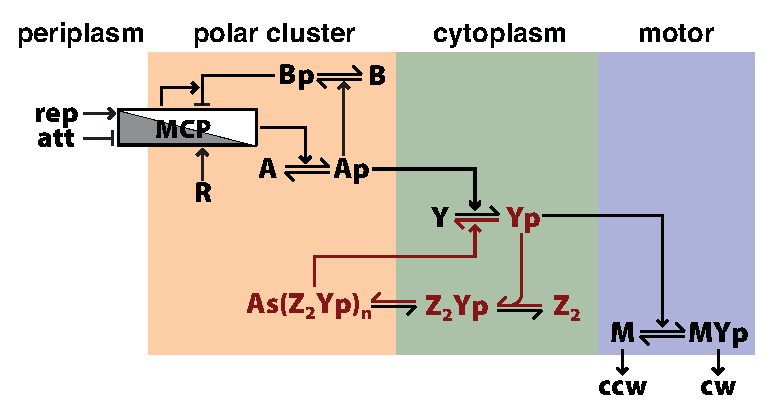
\includegraphics[scale=1]{\docroot introduction/figs/chemotaxis-local-feedback}}
\caption[Modified chemotaxis network]{The chemotaxis network with and without the proposed CheZ feedback loop, from \citet{lipkowfigs}}
\label{fig:intro:netwok}
\end{center}
\end{figure}
\newpage
\subsection{Microscopy}

Microscopy is a rapidly changing field, with advancements coming from all areas. Improvements in optics are yielding diminishing returns in increasing optical resolution, but new illumination and image processing techniques are allowing for finer and finer imaging using otherwise standard equipment, and most manufacturers are now emphasising this area of development more and more in their brochures.

\subsubsection{Localisation Microscopy}
In the context of our challenge - localising proteins and determining density - it would be ideal if we could locate each protein within the \ecoli cell. However, as an \ecoli cell is normally not more than \SI{1}{\micro\meter} in its smallest dimension, and the optical resolution of the microscope is on the order of \SI{200}{\nano\meter}, this is unfeasible using epifluorescent techniques. However, by activating a small subset of all the fluorophores stochastically, identifying each fluorescent point as a fluorescently labelled protein it is possible to build up a composite picture of all the proteins. This has already been demonstrated to work for \ecoli chemotaxis receptors~\citep{greenfield09}.

This stochastic illumination can be achieved in three ways. In Stochastic Optical Reconstruction Microscopy (STORM) or Photo-Activated Localisation Microscopy (PALM), a photo-switching fluorophore is required. A weak activation laser is used such that only a few fluorophores at a time are activated; these are then read off by normal excitation illumination. In Ground State Depletion Microscopy (GSD), `normal' fluorophores are used but a very powerful bleaching laser forces all but a few of them back to the ground state before they have a chance to fluoresce, achieving the same effect (Figure~\ref{fig:advtech:stormpalm}).

STORM, PALM and GSD all require highly sensitive and very fast cameras. They do not require very high resolution optics however, as all that is taken from the optics is the location of a 2D Gaussian. Even so, the higher the resolution the more fluorophores can be imaged simultaneously and the shorter each capture takes. The number of frames required for an image to be built up varies depending on how many fluorophores are being imaged - the more frames the better - but 10,000 is considered to be a reasonable number. Even with some of the fastest cameras available today this would take several seconds.

The image processing techniques required to convert the set of images into a set of locations do not require advanced mathematical knowledge, but do require some understanding of signal processing techniques. Many microscope manufacturers are beginning to offer their own software to do this processing.

\subsubsection{STED Microscopy}

Stimulated Emission Depletion (STED) microscopy is an extension of confocal microscopy that improves the resolution from the norm of around \SI{200}{\nano\meter} to, depending on equipment used, less than \SI{10}{\nano\meter}~\citep{rittweger09}. By depleting a region around the excitation laser its effective diameter is reduced, hence increasing the resolution (Figure~\ref{fig:advtech:sted}).

\subsubsection{TIRF Microscopy}

As this project is looking at proteins localised near the membrane of the cell, Total Internal Reflectance Fluorescence (TIRF) was hoped to be an ideal technique. TIRF allows you to image only the closest \SIrange{50}{200}{\nano\meter} of the sample, removing a lot of background noise (Figure~\ref{fig:advtech:tirf}).

\begin{figure}
\begin{center}
\subfloat[Localisation Microscopy]{
	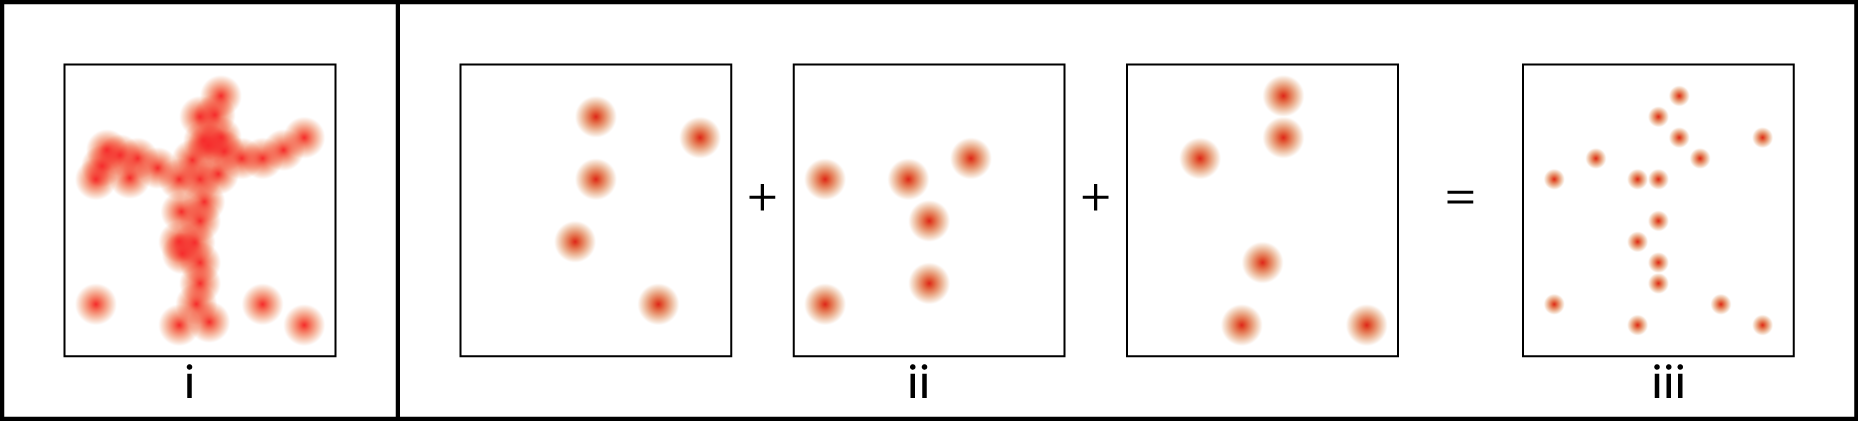
\includegraphics[scale=1]{\docroot introduction/figs/stormpalm.png}
	\label{fig:advtech:stormpalm}
}\\
\subfloat[STED]{
	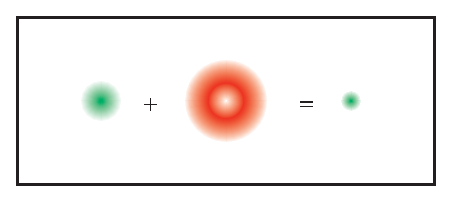
\includegraphics[scale=1]{\docroot introduction/figs/sted}
	\label{fig:advtech:sted}
}
\subfloat[TIRF]{
	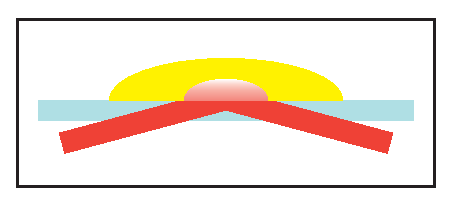
\includegraphics[scale=1]{\docroot introduction/figs/tirf}
	\label{fig:advtech:tirf}
}
\caption[Three advanced microscopy techniques]{Depiction of three advanced microscopy techniques.

\subref{fig:advtech:stormpalm}: Localisation Microscopy. A small subset of the fluorophores fluoresce. In (i) we see a representation of what the image miht look like under epifluorescence. Thousands of images are taken of different subsets of fluorophores (ii). The images may then be processed and each fluorophore localised, allowing for the detection of otherwise unresolvable fine structures (iii).

\subref{fig:advtech:sted}: STED microscopy. Colours are representative. The activation laser (green) is focussed to its smallest size, around \SI{200}{\nano\meter}. A high power redder laser (red) is formed into a doughnut shape and superimposed. This redder laser depletes any excited fluorophores before they can fluoresce, except in the gap in the middle. This gives an effective excitation spot size down to less than \SI{10}{\nano\meter}~\citep{rittweger09}.

\subref{fig:advtech:tirf}: TIRF microscopy. The laser (red) is shone at an extremely oblique angle at the sample through the coverslip (blue). The laser totally internally reflects, forming a decaying evanescent wave (red gradient) in the sample (yellow). The wave is strongest closest to the coverslip, and penetrates further the less oblique the angle, reaching a maximum just before the laser stops reflecting internally, usually at around \SI{200}{\nano\meter}.}
\end{center}
\end{figure}

\subsubsection{FRET Microscopy}
As opposed to localisaiton microscopy, which measure the location of fluorophores and then infer the density, it is possible to measure the density of a population directly. F\"orster Resonance Energy Transfer (FRET) is more commonly used to determine the coincidence of two different fluorophores (Hetero-FRET), but it can also be used to determine the coincidence of two identical fluorophores (Homo-FRET).

\begin{figure}
\begin{center}
\subfloat[Normal fluorophore activity]{
	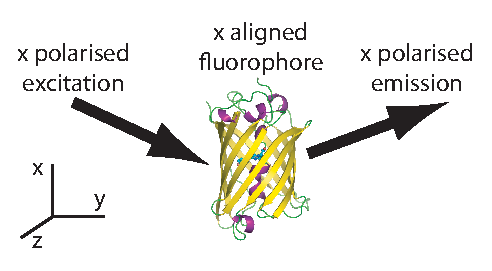
\includegraphics[scale=1]{\docroot introduction/figs/fluorophore}
	\label{fig:fret:normal}
}\\
\subfloat[Homo-FRET]{
	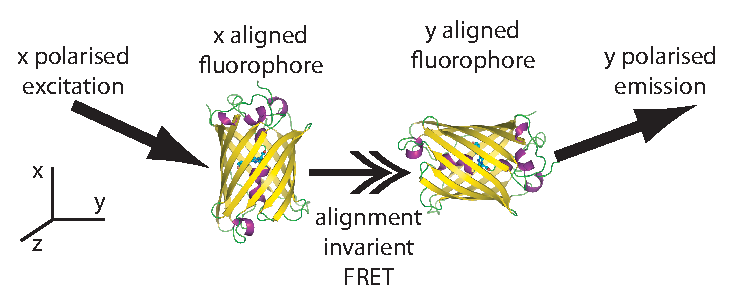
\includegraphics[scale=1]{\docroot introduction/figs/homofret}
	\label{fig:fret:homofret}
}
\caption[Homo-FRET]{Depiction of homo-FRET.

In Figure~\subref{fig:fret:normal}, we see a fluorophore being excited by light polarised in the same plane as its alignment. Light not in this polarisation will not excite the fluorophore. After a short delay, the fluorophore emits light in the same polarisation as its current alignment; usually the same as excitation assuming the fluorophore has not moved much.

In Figure~\subref{fig:fret:homofret}, we see a fluorophore being excited by light polarised in the same plane as its alignment. It then transfers this excitation through FRET to another fluorophore in close proximity to it. This second fluorophore could be in any alignment. The second fluorophore then emits light polarised in the same polarisation as its current alignment; this is now invariant of the original polarisation.}
\label{fig:fret}
\end{center}
\end{figure}

Hetero-FRET measures the conversion of excitation of one fluorophore to the emission of a different type of fluorophore, with the signal from the two fluorophores separated by coloured filters. Homo-FRET uses only one fluorophore, and the standard fluorescence and homo-FRET fluorescence signals are separated by rotating linear polarising filters. Homo-FRET results in a degree of cross-polarised light being emitted from the sample, which corresponds to the number of fluorophores in close proximity to each other. This technique requires monomeric fluorophores that do not spin too fast. If they do, it is likely that some will be excited by the polarised light, but by the time they fluoresce will have spun into a cross-polarised orientation, giving a false signal.
\newpage
\subsection{Gibson Assembly}

Gibson Assembly was developed by Daniel Gibson~\citep{gibson09} in 2009 whilst working with J. Craig Venter on his synthetic genome~\citep{venter10}. In brief, it allows for sequence independent seamless assembly of multiple lengths of DNA. The process requires short (\SIrange{20}{40}{\base}) homologous overlaps between each length to be assembled. These can be created using PCR, as described in Figure~\ref{fig:gibsonPCR}.
\begin{figure}[p]
\subfloat[Two ends of DNA to be joined, in green and blue.]{
\shortstack[l]{
\texttt{\color{DarkGreen}...TCTGGAATTCGCGGCCGCTTCTAGAG-3'\color{black}\ \ \ \ \ \ \ \color{DarkBlue}5'-TACTAGTAGCGGCCGCTGCAGTCCGG...}\\
\texttt{\color{DarkGreen}...AGACCTTAAGCGCCGGCGAAGATCTC-5'\color{black}\ \ \ \ \ \ \ \color{DarkBlue}3'-ATGATCATCGCCGGCGACGTCAGGCC...}
}
\label{fig:gibsonPCR:before}
}\\
\subfloat[Primers required to create overlap in brown, in this case giving an overlap of \SI{24}{\base}.]{
\shortstack[l]{
\texttt{\color{DarkGreen}...TCTGGAATTCGCGGCCGCTTCTAGAG-3'\color{black}}\\
\texttt{\color{DarkRed}\ \ \ \ \ \ \ \ \ < < \ 3'-GGCGAAGATCTCTACTAGTAGCGGCC-5'\color{black}}
\\\\
\texttt{\color{DarkRed}\ \ \ \ \ \ \ \ \ \ \  \ \  \ 5'-CCGCTTCTAGAGATGATCATCGCCGG-3' > >\color{black}}
\\
\texttt{\color{DarkBlue}~~~~~~~~~~~~~~~~~~~~~~~~~~3'-ATGATCATCGCCGGCGACGTCAGGCC...}
}
\label{fig:gibsonPCR:primer}
}
\caption[Primer design for Gibson Assembly]{Depiction of the primers required to create overlap between two strands of arbitrary DNA For each strand of DNA, another primer is required at its other end, which may be either a normal primer if no further assembly is required, or another extension primer as appropriate. Figure adapted from BBF RFC57~\citep{rfc57}.}
\label{fig:gibsonPCR}
\end{figure}

Once this overlap has been created, the lengths of DNA may be assembled in a single isothermal step, as shown in Figure~\ref{fig:gibson}. The enzymes used are T5 exonuclease, Phusion\textregistered\xspace polymerase and Taq ligase. 

\begin{figure}[p]
\centering
\subfloat[Starting DNA with overlaps.]{
\shortstack[l]{
\texttt{\color{DarkGreen}...TCTGGAATTCGCGGCCGCTTCTAGAG\color{RubineRed}TACTAGTAGCGGCCGC-3'}
\\
\texttt{\color{DarkGreen}...AGACCTTAAGCGCCGGCGAAGATCTC\color{RubineRed}ATGATCATCGCCGGCG-5'}
\\
\texttt{\color{RubineRed}\ \ \ \ \ \ \ \ \ \ 5'-GCGGCCGCTTCTAGAG\color{DarkBlue}TACTAGTAGCGGCCGCTGCAGTCCGG...}
\\
\texttt{\color{RubineRed}\ \ \ \ \ \ \ \ \ \ 3'-CGCCGGCGAAGATCTC\color{DarkBlue}ATGATCATCGCCGGCGACGTCAGGCC...}
}
\label{fig:gibson:1}
}\\
\subfloat[DNA is chewed back from 5' end by exonuclease]{
\shortstack[l]{
\texttt{\color{DarkGreen}...TCTGGAATTCGCGGCCGCTTCTAGAG\color{RubineRed}TACTAGTAGCGGCCGC-3'}
\\
\texttt{\color{DarkGreen}...AGA-5'\color{black}<--}
\\
\texttt{\color{DarkBlue}\ \ \ \ \ \ \ \ \ \ \ \ \ \ \ \ \ \ \ \ \ \ \ \ \ \ \ \ \ \ \ \ \ \ \ \ \ \ \ \ \ \ \ \ \ \ \color{black}-->\color{DarkBlue}5'-CGG...}
\\
\texttt{\color{RubineRed}\ \ \ \ \ \ \ \ \ \ 3'-CGCCGGCGAAGATCTC\color{DarkBlue}ATGATCATCGCCGGCGACGTCAGGCC...}
}
\label{fig:gibson:2}
}\\
\subfloat[The two sticky ends anneal]{
\shortstack[l]{
\texttt{\color{DarkGreen}...TCTGGAATTCGCGGCCGCTTCTAGAG\color{RubineRed}TACTAGTAGCGGCCGC-3'\ \color{DarkBlue}5'-CGG...}
\\
\texttt{\color{DarkGreen}...AGA-5'\ \color{RubineRed}3'-CGCCGGCGAAGATCTC\color{DarkBlue}ATGATCATCGCCGGCGACGTCAGGCC...}
}
\label{fig:gibson:3}
}\\
\subfloat[The gaps are filled in by polymerase]{
\shortstack[l]{
\texttt{\color{black}\ \ \ \ \ \ \ \ \ \ \ \ \ \ \ \ \ \ \ \ \ \ \ \ \ \ \ \ \ \ \ \ \ \ \ \ \ \ \ \ \ \ \ \ \ -->\ \ \ \ }
\\
\texttt{\color{DarkGreen}...TCTGGAATTCGCGGCCGCTTCTAGAG\color{RubineRed}TACTAGTAGCGGCCGC\color{YellowOrange}TGCAGTC\color{DarkBlue}CGG...}
\\
\texttt{\color{DarkGreen}...AGA\color{YellowOrange}CCTTAAG\color{RubineRed}CGCCGGCGAAGATCTC\color{DarkBlue}ATGATCATCGCCGGCGACGTCAGGCC...}
\\
\texttt{\color{black}\ \ \ \ \ \ \ \ \ \ <--}
}
\label{fig:gibson:4}
}\\
\subfloat[The gaps are ligated by ligase]{
\shortstack[l]{
\texttt{\color{black}\ \ \ \ \ \ \ \ \ \ \ \ \ \ \ \ \ \ \ \ \ \ \ \ \ \ \ \ \ \ \ \ \ \ \ \ \ \ \ \ \ \ \ \ ><}
\\
\texttt{\color{DarkGreen}...TCTGGAATTCGCGGCCGCTTCTAGAG\color{RubineRed}TACTAGTAGCGGCCGC\color{YellowOrange}TGCAGTC\color{DarkBlue}CGG...}
\\
\texttt{\color{DarkGreen}...AGA\color{YellowOrange}CCTTAAG\color{RubineRed}CGCCGGCGAAGATCTC\color{DarkBlue}ATGATCATCGCCGGCGACGTCAGGCC...}
\\
\texttt{\color{black}\ \ \ \ \ ><\ \ \ }
}
\label{fig:gibson:5}
}
\caption[Overview of the Gibson Assembly Process]{Overview of the Gibson Assembly Process. Green and blue sequences  represents the two templates. Pink sequences represents PCR extension, and orange sequences represents bases added during the Gibson Assembly Process. All steps occur in the same isothermal reaction. Figure adapted from BBF RFC 57~\citep{rfc57}.}
\label{fig:gibson}
\end{figure}

\subsection{Objective}
It is the objective of this project to test whether CheZ dynamically clusters to the pole of \ecoli cells in response to a chemotactic stimulant. A significant portion of this project will be devoted to determining the most appropriate microscopy technique. The stimulant will be a chemical attractant or repellent; or blue light at \SI{440}{\nano\meter}~\citep{wright06}, which is a repellent to the cells. Levels of chemical chemotactic stimulant will be varied using a microfluidic device.

The primary challenges of this project are threefold:
\begin{enumerate}
\item Determine the most appropriate microscopy technique and implement it
\item Design and implement a microfluidics set-up for media exchange
\item Design and create \ecoli strains with the necessary protein fusions
\end{enumerate}

The secondary challenges of this project include
\begin{enumerate}
\item Replicate homo-FRET results for clustering of Tar proteins
\item Develop image processing tools for high throughput cluster identification
\item Develop image processing tools for high throughput anisotropy
\end{enumerate}


\end{document}